
\documentclass{article}
\usepackage[utf8]{inputenc}
\usepackage[margin=1in,left=1.5in,includefoot]{geometry}
\usepackage{booktabs}
\usepackage{graphicx}
\usepackage{tikz}
\usepackage{amsmath}
\usepackage{ulem}
\usepackage{hyperref}  % Needed for \href
\usetikzlibrary{arrows.meta, positioning, shapes.geometric, fit}
% Header & Footer Stuff

\usepackage{fancyhdr}
\pagestyle{fancy}
\lhead{SPR200: ASSIGNMENT 1}
\rhead{04/12/2025}
\fancyfoot{}
\lfoot{CREATED BY ZAKARIYA OUTBIH, SENECA POLYTECHNIC}
\fancyfoot[R]{}

% The Main Document
\begin{document}

\begin{center}
 \LARGE\bfseries Assignment 1 
 \line(1,0){430}
\end{center}

\begin{center}
 \textbf{Course Number:} SPR200 \\
 \textbf{Course Name:} Basic Cryptography \\
 \textbf{Course Section:} NAA \\
 \textbf{Assignment Number:} 1 \\
 \textbf{Student Full Name:} Zakariya Outbih \\
 \textbf{Student GitHub Username:} zoutbih\_seneca
\end{center}

\section*{Feistel Cipher Diagrams}

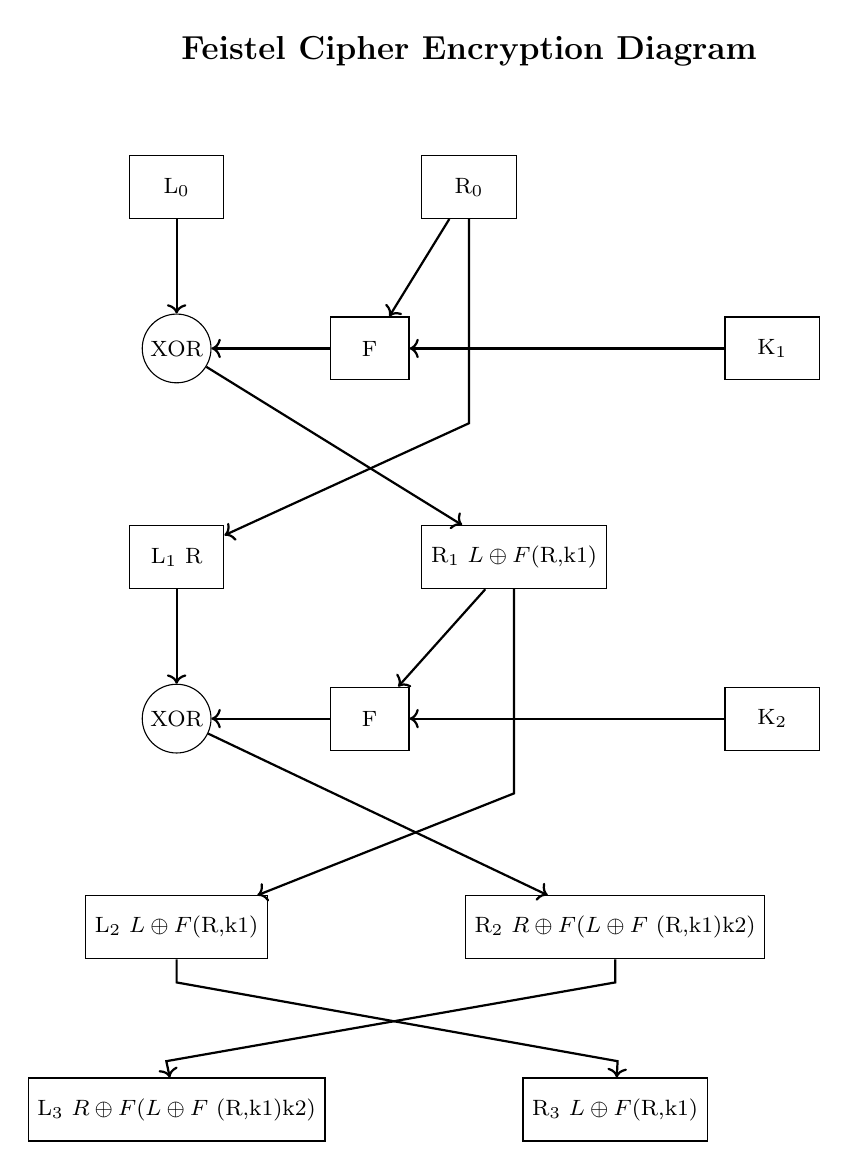
\begin{tikzpicture}[
    box/.style = {draw, minimum width=1.2cm, minimum height=0.8cm},
    xor/.style = {circle, draw, inner sep=2pt},
    fbox/.style = {draw, minimum width=1cm, minimum height=0.8cm},
    dashedbox/.style = {draw, dashed, inner sep=0.2cm, rounded corners},
    arrow/.style = {->, thick},
    every node/.style={font=\footnotesize}
  ]
  

  % Initial inputs
  \node[box] (L0) {L\textsubscript{0}};
  \node[box, right=2.5cm of L0] (R0) {R\textsubscript{0}};
  
%Title
\node[above=1cm of R0, font=\bfseries\large] (title) {Feistel Cipher Encryption Diagram};
  
  % XOR and F for Round 1
  \node[xor, below=1.2cm of L0] (xor1) {XOR};
  \node[fbox, right=1.5cm of xor1] (f1) {F};
  \node[box, right=4cm of f1] (k1) {K\textsubscript{1}};
  
  % L1 and R1
  \node[box, below=1.8cm of xor1] (L1) {L\textsubscript{1} R};
  \node[box, right=2.5cm of L1] (R1) {R\textsubscript{1}  $L \oplus F$(R,k1)};
  
  % Arrows Round 1
  \draw[arrow] (R0) -- (f1);
  \draw[arrow] (k1) -- (f1);
  \draw[arrow] (f1) -- (xor1);
  \draw[arrow] (L0) -- (xor1);
  \draw[arrow] (xor1) -- (R1);
  \draw[->, thick]
  (R0) -- ++(0,-3)    % down
       -- (L1);       % into L1
  

  
  % Round 2
  
  
  % XOR F and k1
  \node[xor, below=1.2cm of L1] (xor2) {XOR};
  \node[fbox, right=1.5cm of xor2] (f2) {F};
  \node[box, right=4cm of f2] (K2) {K\textsubscript{2}};
  
  % L2 and R2
  \node[box, below=1.8cm of xor2] (L2) {L\textsubscript{2} $L \oplus F$(R,k1)};
  \node[box, right=2.5cm of L2] (R2) {R\textsubscript{2} $R \oplus F$($L \oplus F$ (R,k1)k2)};

  % L3 and R3
  \node[box, below=1.5cm of L2] (L3) {L\textsubscript{3} $R \oplus F$($L \oplus F$ (R,k1)k2)};
  \node[box, below=1.5cm of R2] (R3) {R\textsubscript{3}  $L \oplus F$(R,k1)};
  
  % Arrows Round 2
  \draw[arrow] (R1) -- (f2);
  \draw[arrow] (K2) -- (f2);
  \draw[arrow] (f2) -- (xor2);
  \draw[arrow] (L1) -- (xor2);
  \draw[arrow] (xor2) -- (R2);
  \draw[->, thick]
  (R1) -- ++(0,-3)    % down
       -- (L2);       % into L2

\draw[->, thick] 
(R2) -- ++(0,-0.7)         % Step 1: go down a bit
     -- ++(-5.7,-1)          % Step 2: diagonal left-down
     -- (L3);              % Step 3: connect straight to L3

\draw[->, thick] 
(L2) -- ++(0,-0.7)         % Step 1: go down a bit
     -- ++(5.6,-1)          % Step 2: diagonal left-down
     -- (R3);              % Step 3: connect straight to L3

  
  \end{tikzpicture}

    
I first made the encryption diagram to better understand the decryption one. Essentially there is one plaintext given and divided into two parts, L0 and R0. Each round the right side is passed through the function and the left side is xored to the output. The important thing to note is that each round R1, R2, R3 the left and right sides are swapped so R1 becomes L1 and so on.


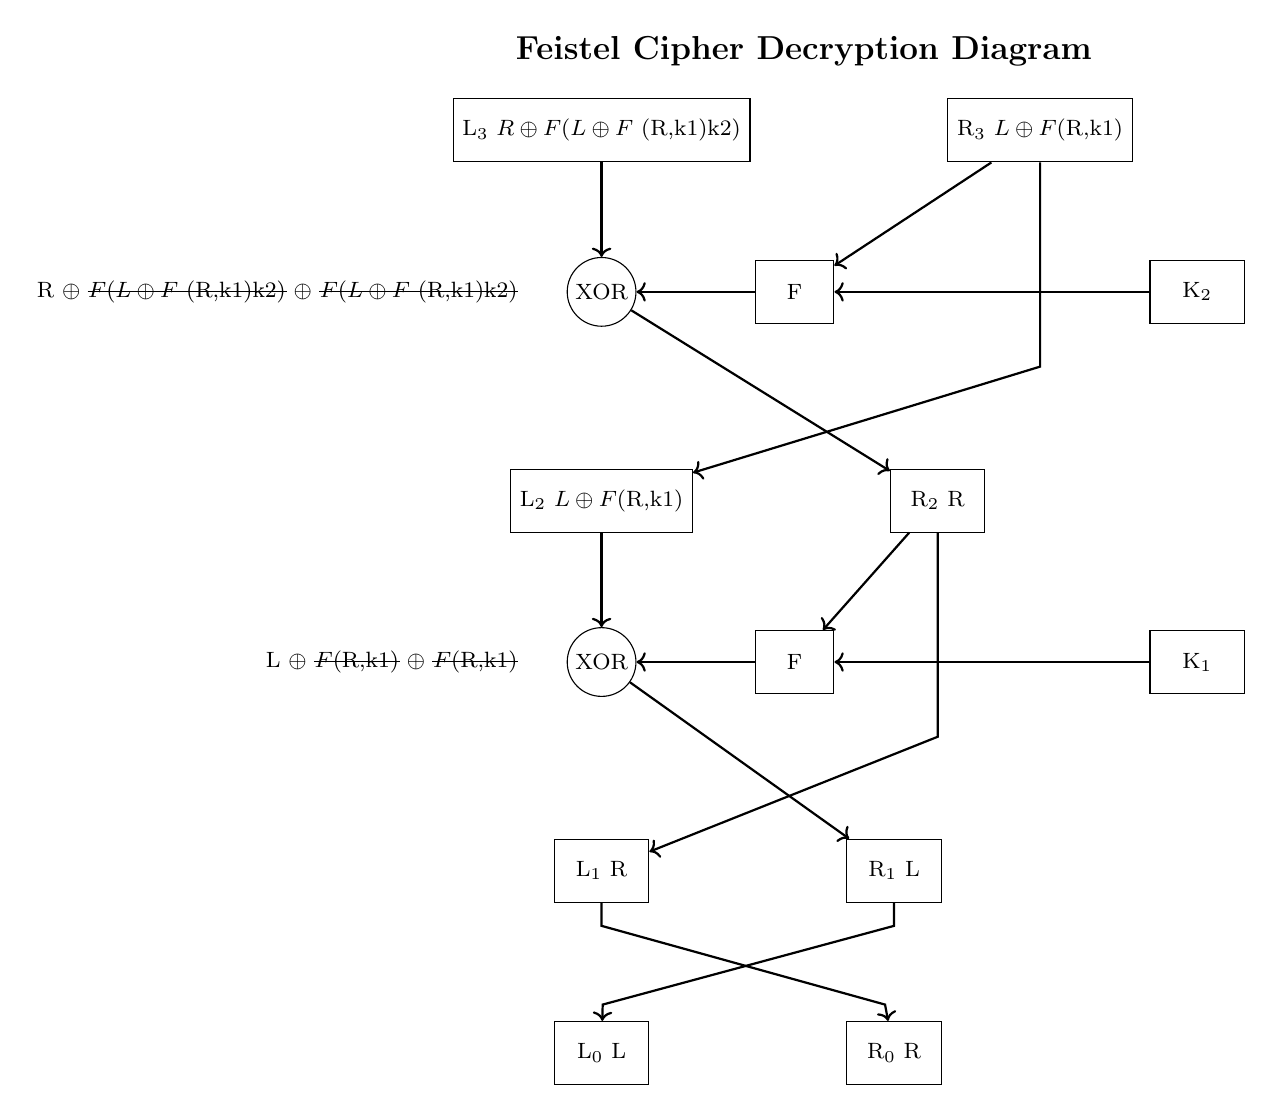
\begin{tikzpicture}[
    box/.style = {draw, minimum width=1.2cm, minimum height=0.8cm},
    xor/.style = {circle, draw, inner sep=2pt},
    fbox/.style = {draw, minimum width=1cm, minimum height=0.8cm},
    dashedbox/.style = {draw, dashed, inner sep=0.2cm, rounded corners},
    arrow/.style = {->, thick},
    every node/.style={font=\footnotesize}
  ]
  

  % Initial inputs
  \node[box] (L0) {L\textsubscript{3} $R \oplus F$($L \oplus F$ (R,k1)k2)};
  \node[box, right=2.5cm of L0] (R0) {R\textsubscript{3} $L \oplus F$(R,k1)};
  
%Title
\node[shift={(-3cm,1cm)},  font=\bfseries\large] (title) at (R0) {Feistel Cipher Decryption Diagram};
  
  % XOR and F for Round 1
  \node[xor, below=1.2cm of L0] (xor1) {XOR};
  \node[fbox, right=1.5cm of xor1] (f1) {F};
% Crossed-out mathematical expression next to XOR block
\node[left=0.5cm of xor1] (text1) {R $ \oplus $ \sout{$F$($L \oplus F$ (R,k1)k2)} $ \oplus $ \sout{$F$($L \oplus F$ (R,k1)k2)}};
\node[box, right=4cm of f1] (k1) {K\textsubscript{2}};
  
  % L2 and R2
  \node[box, below=1.8cm of xor1] (L1) {L\textsubscript{2} $L \oplus F$(R,k1)};
  \node[box, right=2.5cm of L1] (R1) {R\textsubscript{2}  R};
  
  % Arrows Round 1
  \draw[arrow] (R0) -- (f1);
  \draw[arrow] (k1) -- (f1);
  \draw[arrow] (f1) -- (xor1);
  \draw[arrow] (L0) -- (xor1);
  \draw[arrow] (xor1) -- (R1);
  \draw[->, thick]
  (R0) -- ++(0,-3)    % down
       -- (L1);       % into L1
  

  
  % Round 2
  
  
  % XOR F and k1
  \node[xor, below=1.2cm of L1] (xor2) {XOR};
  \node[fbox, right=1.5cm of xor2] (f2) {F};
  % Crossed-out mathematical expression next to XOR block
  \node[left=0.5cm of xor2] (text1) {L $ \oplus $ \sout{$F$(R,k1)} $ \oplus $ \sout{$F$(R,k1)}};
  \node[box, right=4cm of f2] (K2) {K\textsubscript{1}};
  
  % L1 and R1
  \node[box, below=1.8cm of xor2] (L2) {L\textsubscript{1} R};
  \node[box, right=2.5cm of L2] (R2) {R\textsubscript{1} L};

  % L1 and R0
  \node[box, below=1.5cm of L2] (L3) {L\textsubscript{0} L};
  \node[box, below=1.5cm of R2] (R3) {R\textsubscript{0} R};
  
  % Arrows Round 2
  \draw[arrow] (R1) -- (f2);
  \draw[arrow] (K2) -- (f2);
  \draw[arrow] (f2) -- (xor2);
  \draw[arrow] (L1) -- (xor2);
  \draw[arrow] (xor2) -- (R2);
  \draw[->, thick]
  (R1) -- ++(0,-3)    % down
       -- (L2);       % into L2

\draw[->, thick] 
(R2) -- ++(0,-0.7)         % Step 1: go down a bit
     -- ++(-3.7,-1)          % Step 2: diagonal left-down
     -- (L3);              % Step 3: connect straight to L3

\draw[->, thick] 
(L2) -- ++(0,-0.7)         % Step 1: go down a bit
     -- ++(3.6,-1)          % Step 2: diagonal left-down
     -- (R3);              % Step 3: connect straight to L3

  
\end{tikzpicture}

As you can see this diagram (decryption) is essentially the reverse of the Encryption diagram. This is how the Feistel cipher works. It uses the properties of the XOR operation to encrypt and decrypt. You can pass the plain text as many times as you would like through the function + XOR operation and still be able to decrypt the plaintext. In the XOR operation both inputs must be different for the output to be true or (1). Meaning that if the inputs are the same (or part of the inputs are the same) like in the decryption diagram then they cancel each other out.

\vspace{2em} % spacing

Here is a great link from computerphile explaining the feistel cipher in more detail: 
%hyperlink
\href{https://www.youtube.com/watch?v=FGhj3CGxl8I&t=29s}{Click Here};


\vspace{15em} % spacing

% 2-DES and 3-DES Diagram and explanation
\section*{2-DES and 3-DES: Diagrams and Explanation}

\textbf{2-DES:}
\vspace{0.3cm}

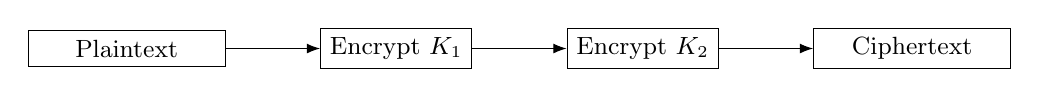
\begin{tikzpicture}[node distance=1.8cm and 1.2cm, every node/.style={font=\small}, >=Latex]

% Nodes
\node (pt) [draw, minimum width=2.5cm] {Plaintext};
\node (e1) [draw, right=of pt, minimum width=1.8cm] {Encrypt $K_1$};
\node (e2) [draw, right=of e1, minimum width=1.8cm] {Encrypt $K_2$};
\node (ct) [draw, right=of e2, minimum width=2.5cm] {Ciphertext};

% Arrows
\draw[->] (pt) -- (e1);
\draw[->] (e1) -- (e2);
\draw[->] (e2) -- (ct);

\end{tikzpicture}

\vspace{0.5cm}
\textbf{Why 2-DES is insecure:} \\
Although 2-DES uses two keys and seems to offer $112$ bits of security ($56 \ bits \times 2$), it is vulnerable to a \textbf{meet-in-the-middle attack}, which reduces the effective security to about $2^{57}$ operations. The attacker can encrypt the plaintext with all possible $K_1$ values and decrypt the ciphertext with all possible $K_2$ values, then match the intermediate results. This makes 2-DES only marginally more secure than DES.

\vspace{0.7cm}
\textbf{3-DES (Encrypt-Decrypt-Encrypt):}
\vspace{0.3cm}

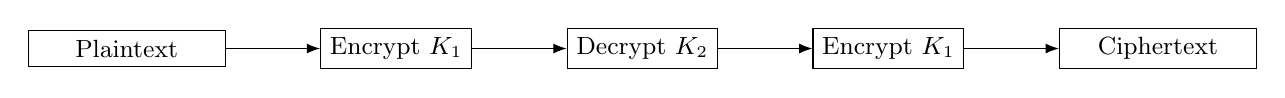
\begin{tikzpicture}[node distance=1.8cm and 1.2cm, every node/.style={font=\small}, >=Latex]

% Nodes
\node (pt3) [draw, minimum width=2.5cm] {Plaintext};
\node (e3_1) [draw, right=of pt3, minimum width=1.8cm] {Encrypt $K_1$};
\node (d3_2) [draw, right=of e3_1, minimum width=1.8cm] {Decrypt $K_2$};
\node (e3_3) [draw, right=of d3_2, minimum width=1.8cm] {Encrypt $K_1$};
\node (ct3) [draw, right=of e3_3, minimum width=2.5cm] {Ciphertext};

% Arrows
\draw[->] (pt3) -- (e3_1);
\draw[->] (e3_1) -- (d3_2);
\draw[->] (d3_2) -- (e3_3);
\draw[->] (e3_3) -- (ct3);

\end{tikzpicture}

\vspace{0.5cm}
\textbf{Why 3-DES is better:} \\
3-DES increases the complexity significantly by applying DES three times — Encrypt with $K_1$, Decrypt with $K_2$, then Encrypt with $K_1$ again. This makes it resistant to the meet-in-the-middle attack and gives an effective security of approximately $112$ bits. The use of decryption in the middle also ensures backward compatibility with single DES when $K_1 = K_2$.

\end{document}